\section{Network Diagram (Precedence Diagram Method)}
Two sets of diagrams have been set. An expanded one \ref{NPM_extended}, to see interconnections between tasks and a brief description and a short one \ref{NPM_short}, to see interconnections betweens activities, only using the id. By doing this, is expected to make easier the tasks visualization.
\begin{landscape}
	\begin{figure}[H]
		\centering
		\begin{tabular}{@{}c@{\hspace{.5cm}}c@{}}
			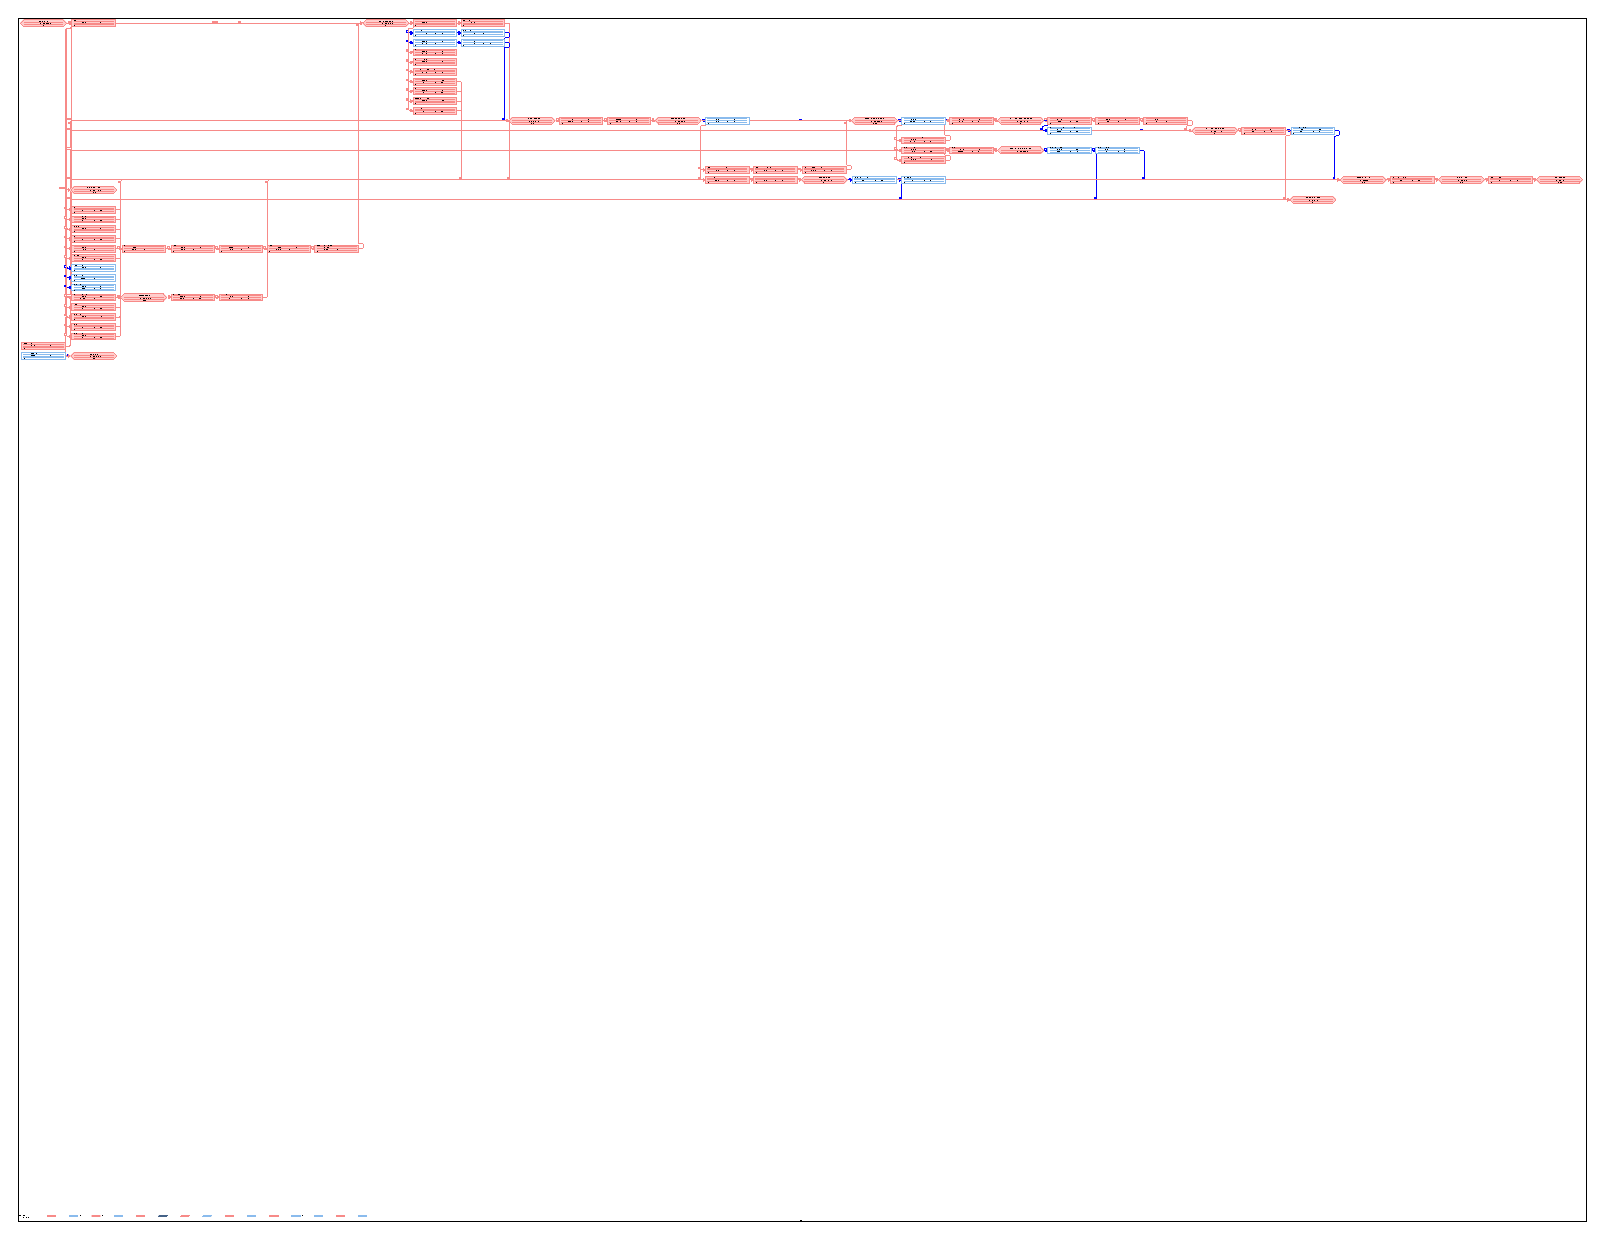
\includegraphics[page=1,width=1.55\textwidth, trim={0 14.5cm 0 0},clip]{./images/gantt/NPM_expanded.pdf}\\
			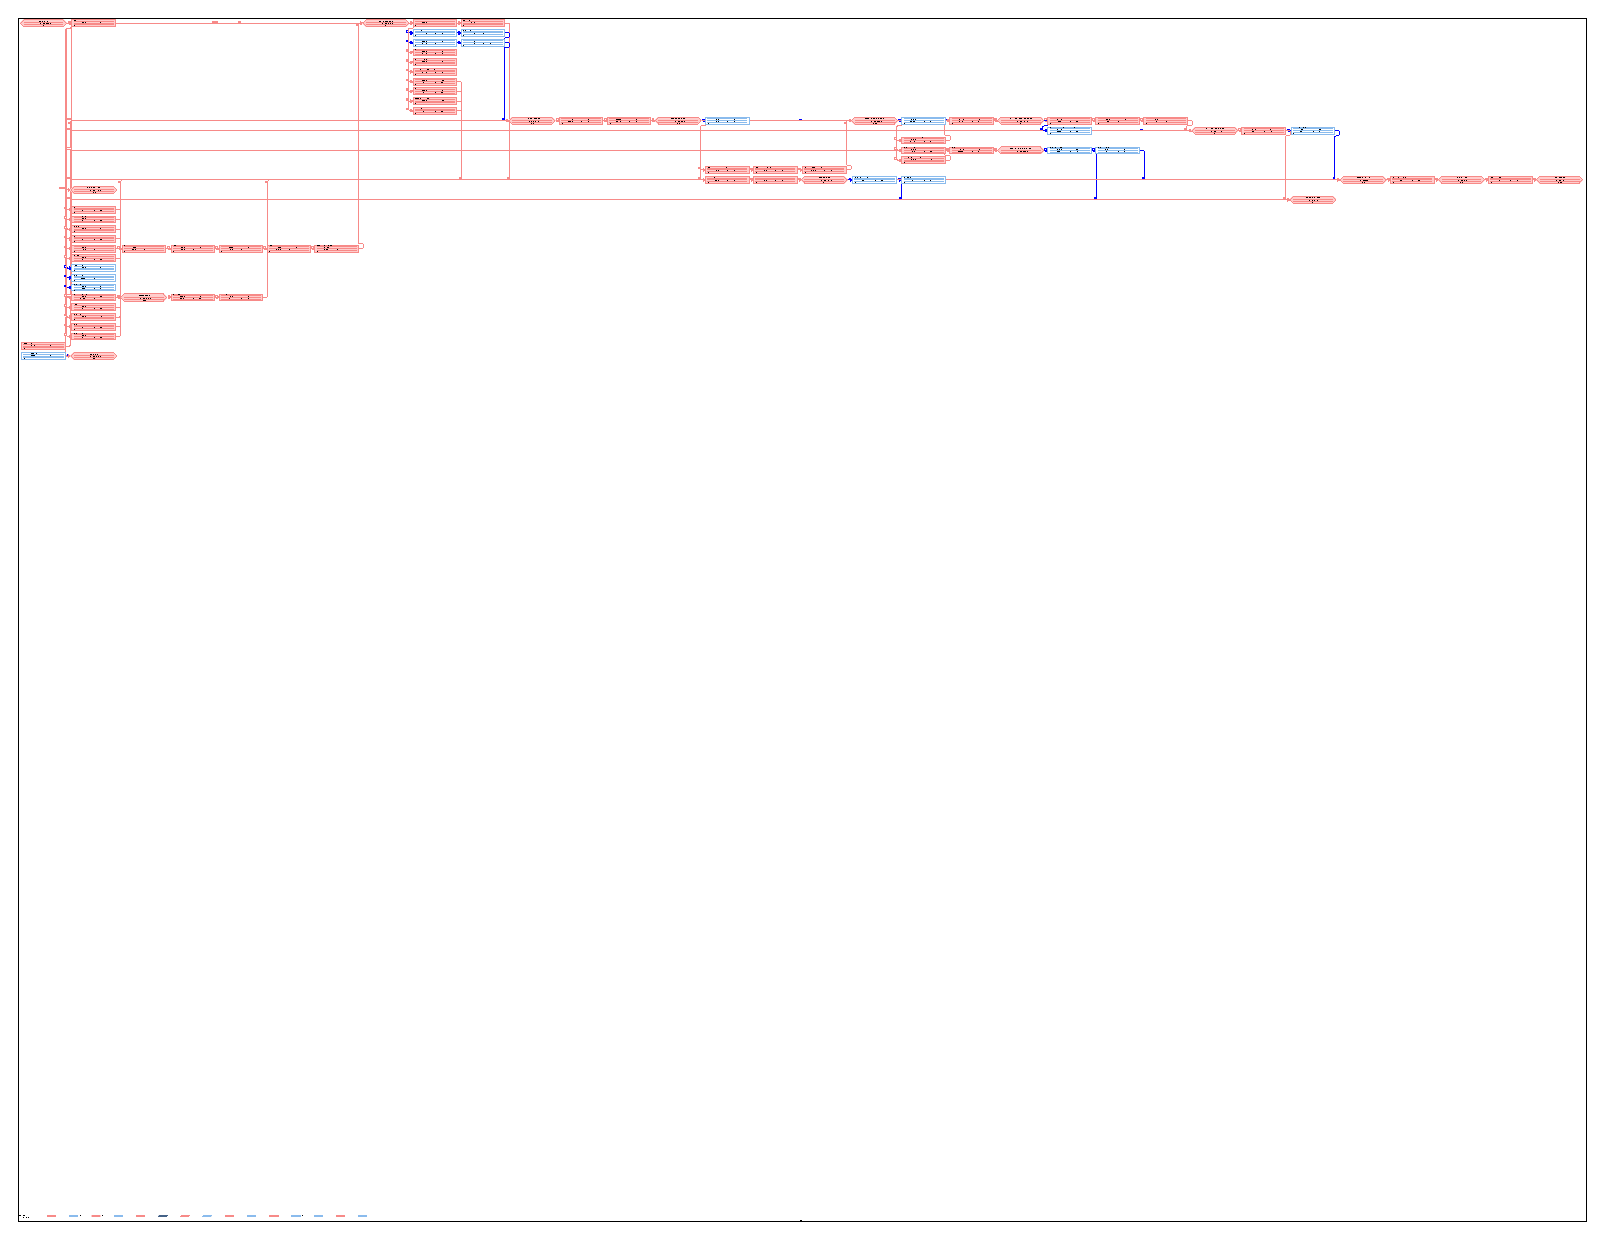
\includegraphics[page=1,width=1.55\textwidth, trim={0 0 0 20cm},clip]{./images/gantt/NPM_expanded.pdf}
		\end{tabular}
		\caption{Network Precedence Method chart with full detail modules.}
		\label{NPM_extended}
	\end{figure}

	\begin{figure}[H]
		\centering
		\begin{tabular}{@{}c@{\hspace{.5cm}}c@{}}
			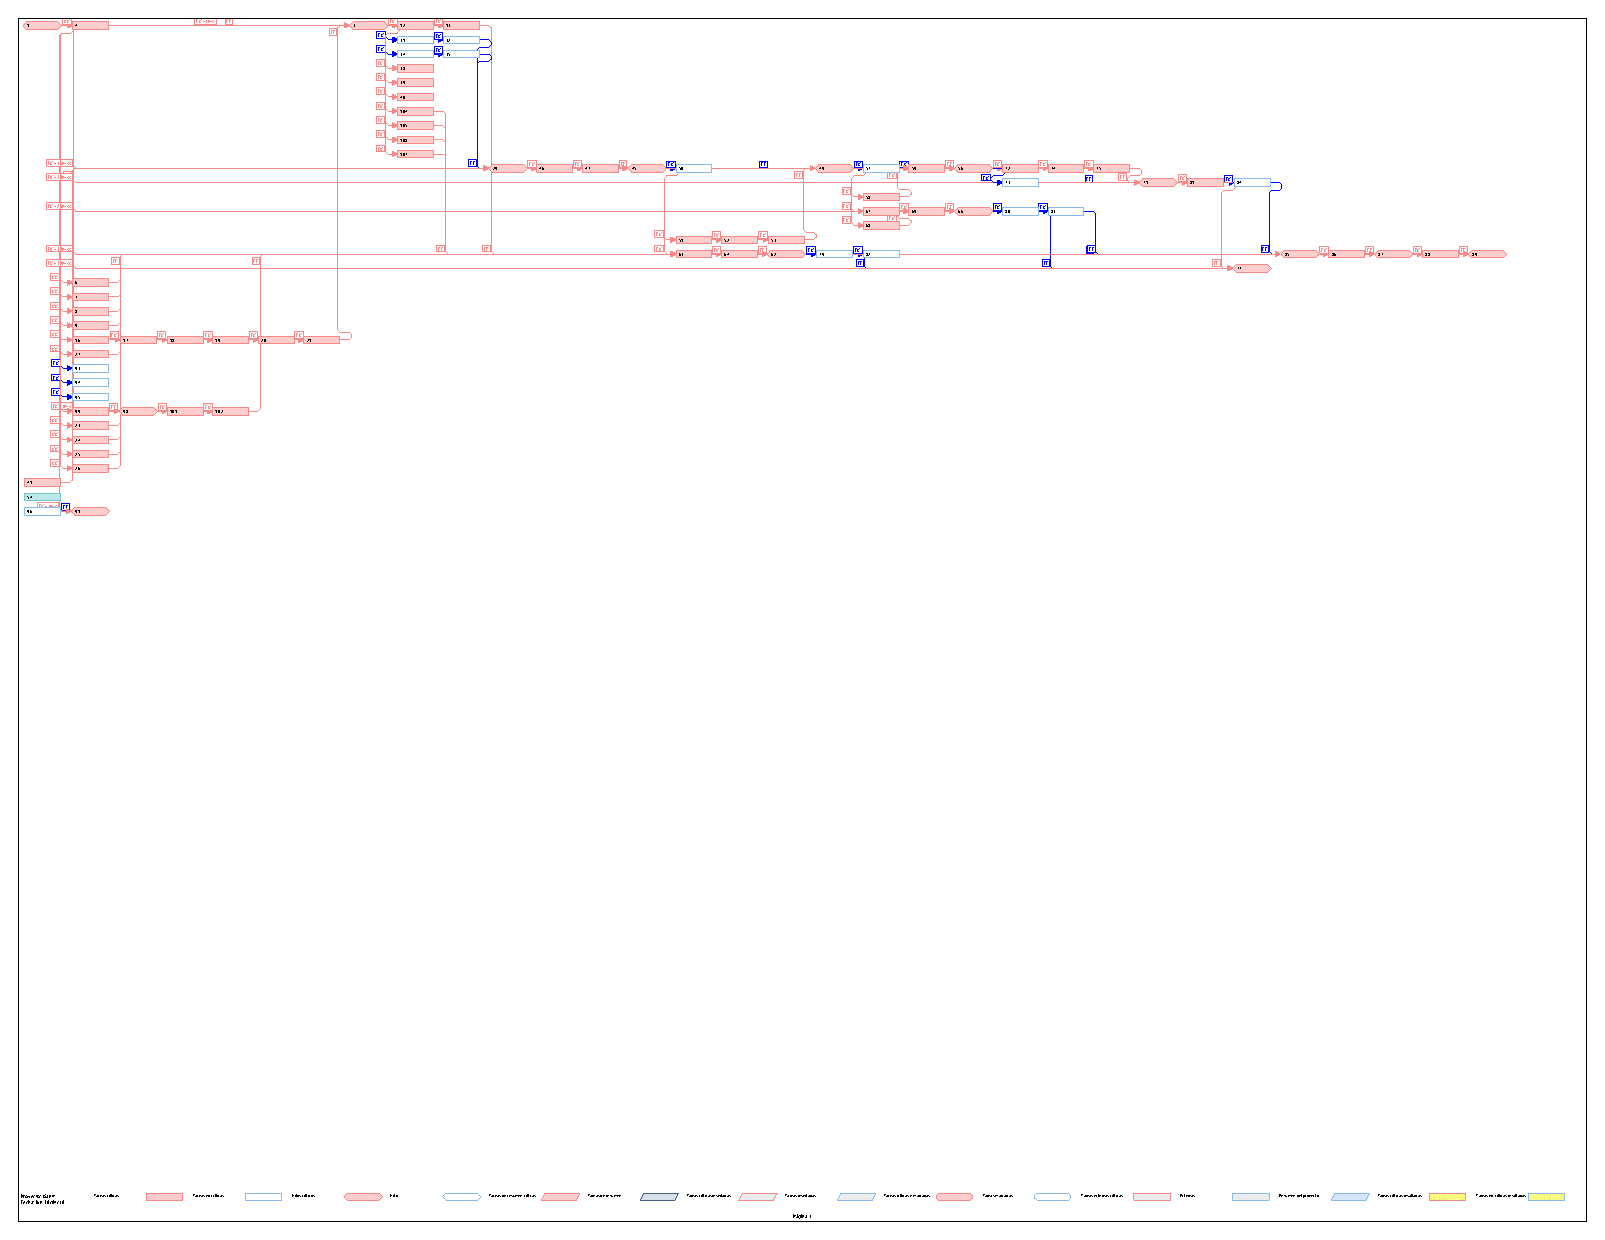
\includegraphics[page=1,width=1.5\textwidth]{./images/gantt/NPM_short.pdf}
		\end{tabular}
		\caption{Network Precedence Method chart with only the tasks identification.}
		\label{NPM_short}
	\end{figure}
\end{landscape}


%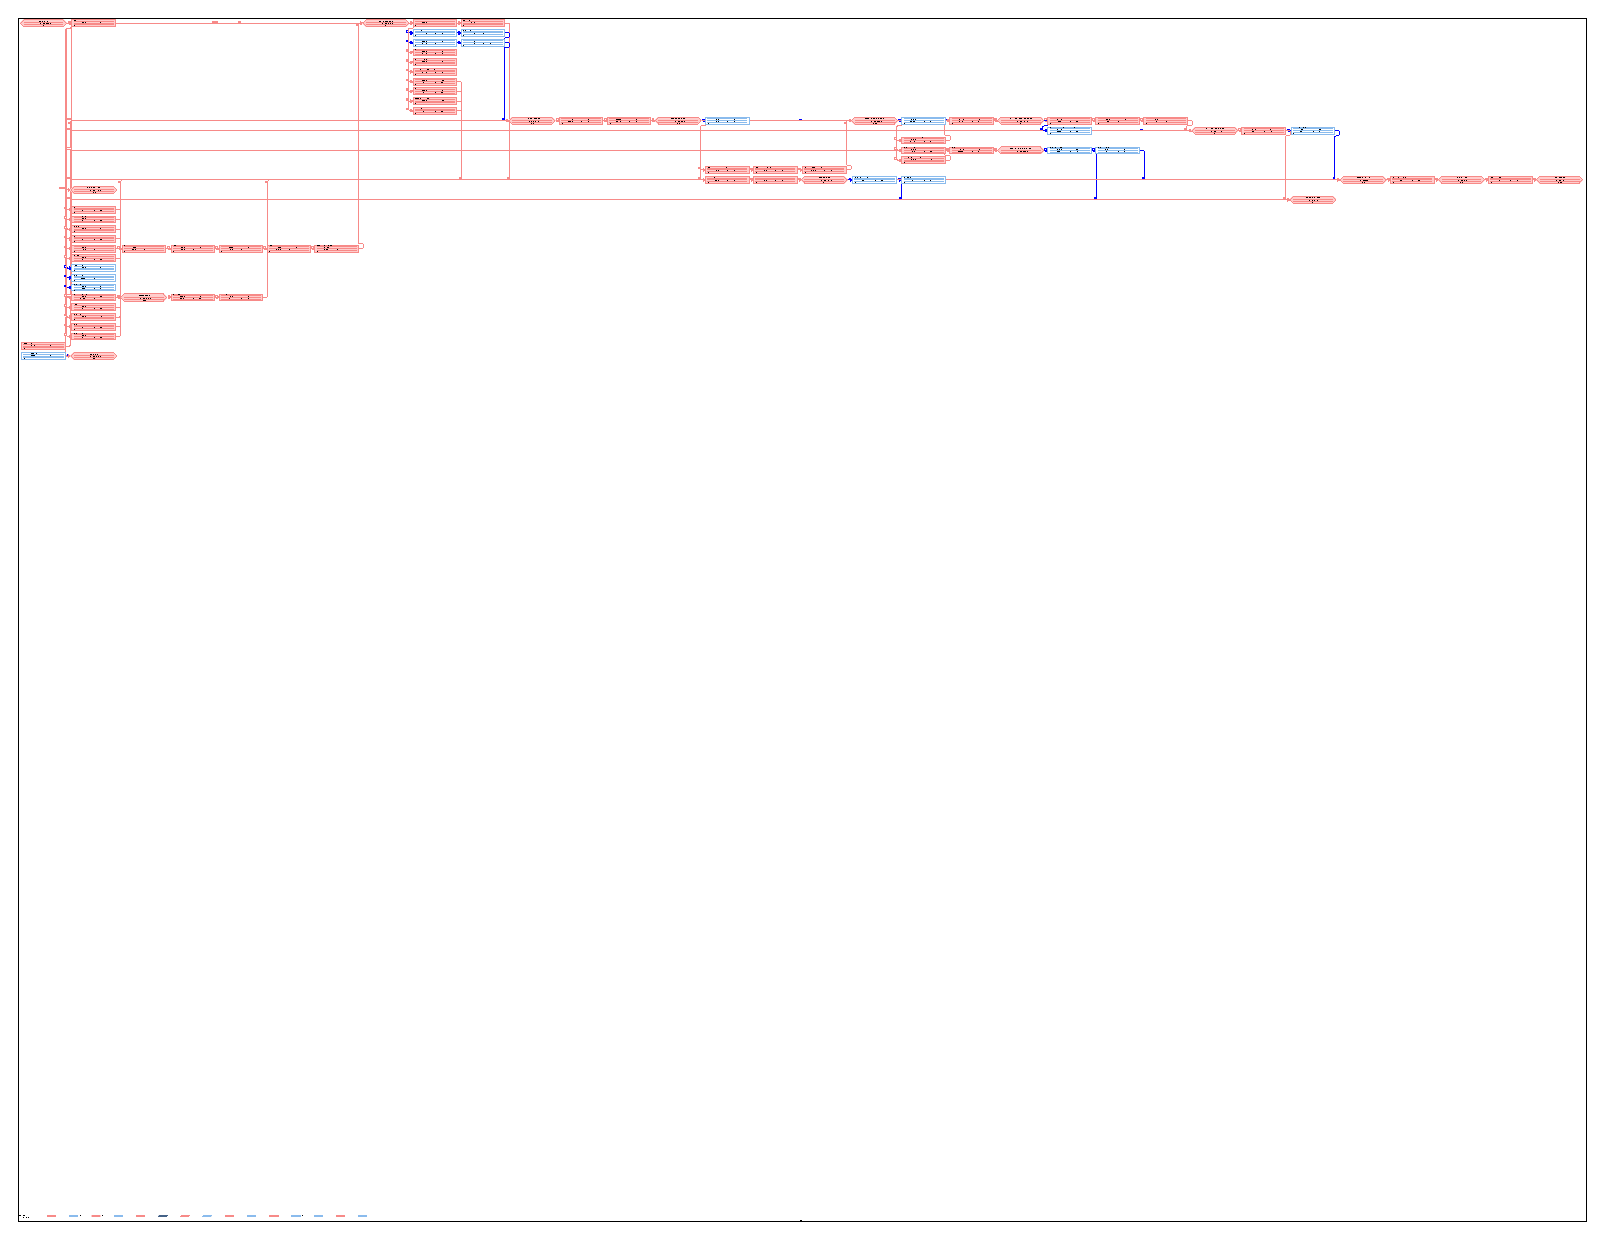
\includepdf[landscape=true]{./images/gantt/NPM_expanded.pdf}
%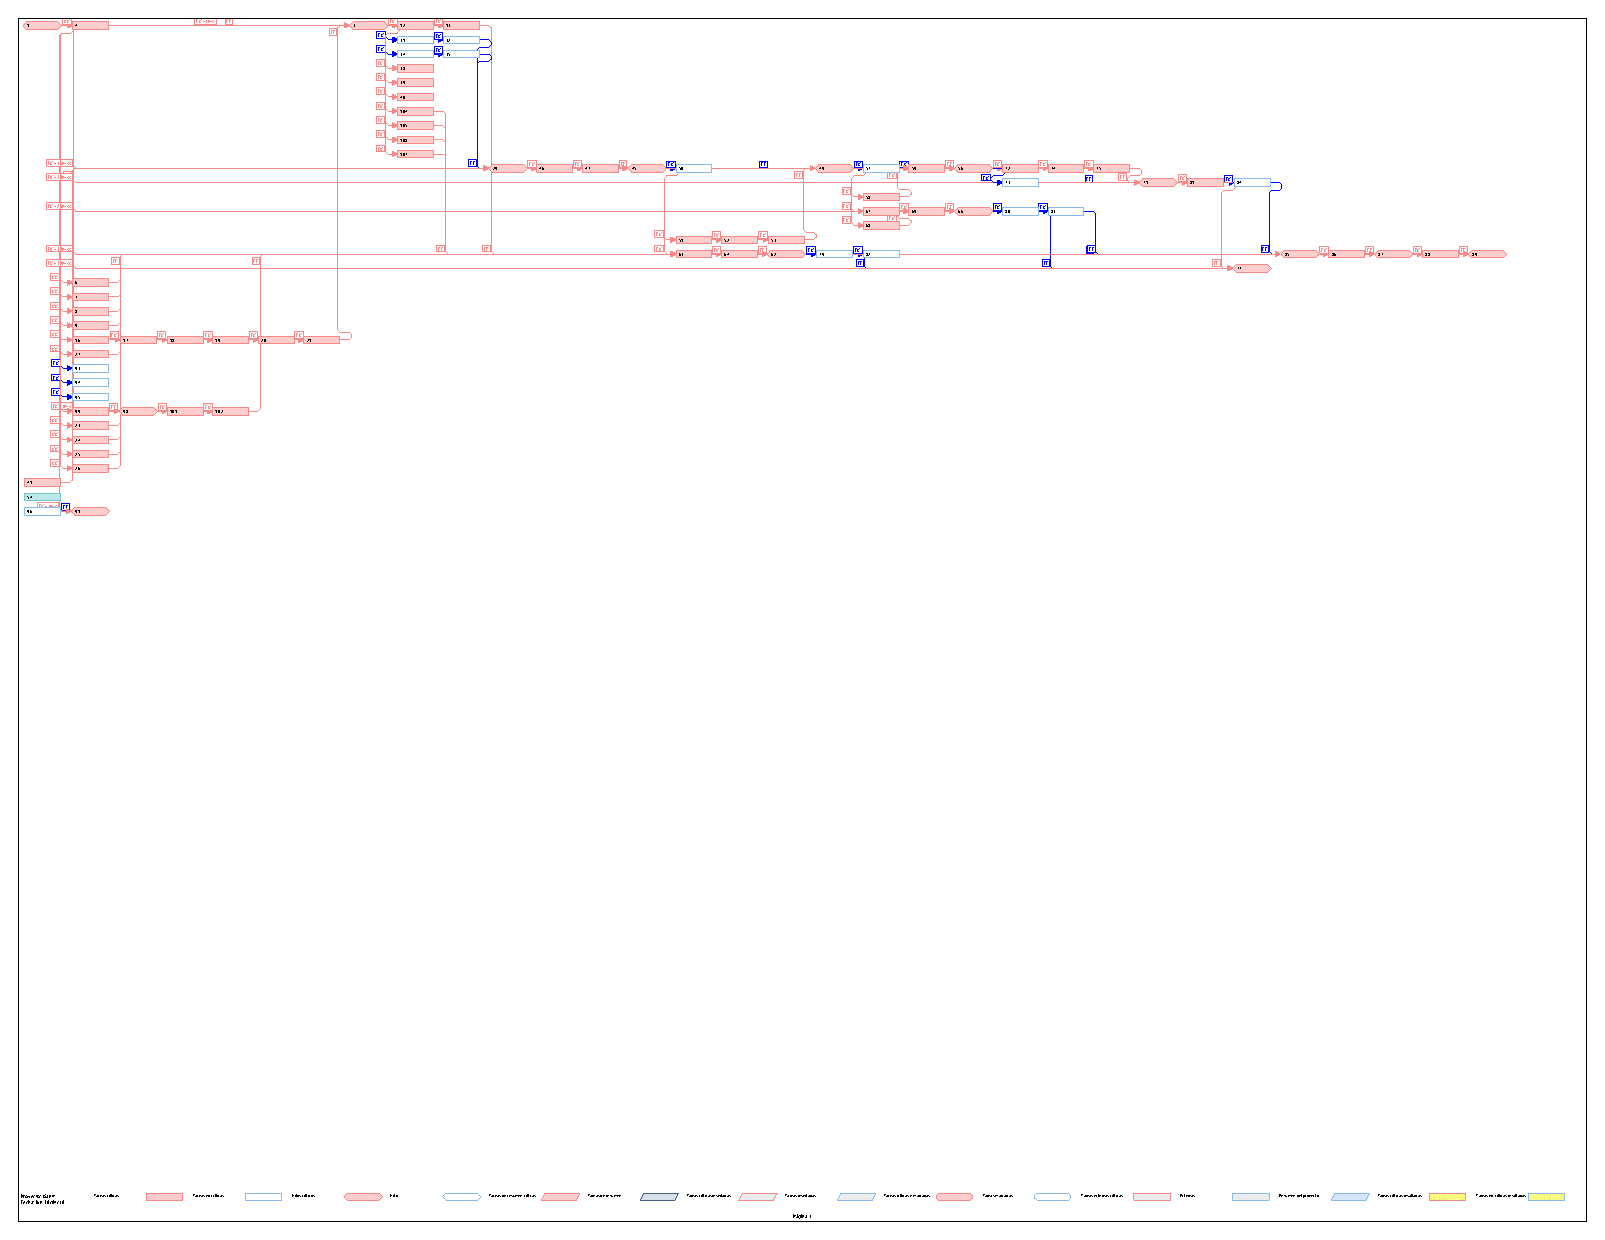
\includepdf[landscape=true]{./images/gantt/NPM_short.pdf}